\pagestyle{plain}

\chapter{Problema da Mochila Compartimentada} \label{sec:compartimentada}

O Problema da Mochila Compartimentada é uma variação do Problema da Mochila. Este problema consiste em determinar as capacidades adequadas de vários compartimentos que podem vir a ser alocados em uma mochila e como esses devem ser carregados, respeitando as capacidades dos compartimentos e da mochila.

\section{Definição do Problema}

Um alpinista deve carregar sua mochila com $m$ possíveis itens de sua utilidade. A cada item $i$, o alpinista atribui um valor de utilidade $b_i$ e seu peso $p_i$. O máximo peso que o alpinista suporta em sua viagem é $L$. Porém, os itens são de agrupamentos distintos e devem estar em compartimentos separados dentro da mochila. Os compartimentos da mochila são flexíveis e as capacidades dos compartimentos são limitados superiormente, caso estes sejam criados, por $L_k$. Cada compartimento tem custo $c_k$ para ser criado e, além disso, cada compartimento criado diminui a capacidade da mochila em $S$.

\subsection{Modelo Matemático}

Considere uma modificação do Problema da Mochila clássico, onde os itens devam ser agrupados em subconjuntos, de modo que, itens de um agrupamento não podem ser mistrudados com itens de outro. O Problema da Mochila Compartimentada consiste em preencher de maneira ótima uma mochila por meio da construção de compartimentos no seu interior, onde cada um deles é formado por itens de um agrupamento. Segue abaixo a formalização deste problema, de acordo com  ~\cite{Mar00}:

\begin{itemize}
	\item $M=\{1,...,m\}$: conjunto dos tipos de itens;
	\item $K$: quantidade de classes distintas (ou partições);
	\item $C_k$: subconjunto de $M$, contendo itens de mesma classe, $k=1,...,K$ (para $i \neq j$, $C_i  \bigcap C_j = \emptyset$);
	\item $c_k$: custo de incluir um compartimento para itens da classe $k$ na mochila ($c_{k} \geq 0$), $k = 1, ..., K$;
	\item $S$: perda decorrente da inclusão de um novo compartimento na mochila;
	\item $L$: capacidade da mochila;
	\item $N_k$: número total de possíveis compartimentos para a classe $k$;
	\item $L_{max}$: capacidade máxima de cada compartimento;
	\item $L_{min}$: capacidade mínima de cada compartimento ($L_{min} < L_{max} < L$);
	\item $l_i$: peso do item $i$ ($l_i >0$), $i = 1, ..., m$; 
	\item $b_i$: benefício ou utilidade do item $i$ ($b_i \geq 0$), $i=1,...,m$;
	\item $d_i$: limite máximo de itens $i$ na mochila, $i = 1, ..., m$;
	\item $\alpha_{ijk}$: número de itens do tipo $i$, da classe $k$, no compartimento do tipo $j$ ($i = 1, ..., m, k = 1, ..., K$ e $j = 1, ..., N_{k}$); e
	\item $\beta_{jk}$ número de repetições do compartimento do tipo $j$ alocados com a classe $k, k = 1, ..., K$ e $j = 1, ..., N_{k}$.
\end{itemize}

Assim, o $j$-ésimo compartimento com itens da classe  $k$ tem:

\begin{itemize}
	\item A capacidade ocupada dada por:
	\begin{eqnarray}
		L_{jk}: \sum_{i \in C_{k}}l_{i}\alpha_{ijk}, & k = 1, ..., K \ e \ j = 1, ..., N_{k}.
	\end{eqnarray}

	\item O valor de utilidade, ou benefício, dado por:
	\begin{eqnarray}
		V_{jk}: \sum_{i \in C_{k}}b_{i}\alpha_{ijk}, & k = 1, ..., K \ e \ j = 1, ..., N_{k}.
	\end{eqnarray}

\end{itemize}

Um modelo matemático para o problema de preencher uma única mochila compartimentada pode ser escrito por:

\begin{eqnarray}
	Maximizar: & \displaystyle \sum_{k = 1}^{K}\sum_{j = 1}^{N_{k}}(V_{jk} - c_{l})\beta_{jk} \\
	Sujeito \ a: &  \displaystyle V_{jk} = \sum_{i \in C_{k}}b_{i}\alpha_{ijk}, \ k = 1, ..., K \ e \ j = 1, ..., N_{k} \\
	& \displaystyle L_{jk} = \sum_{i \in C_{k}}l_{i}\alpha_{ijk}, \ k = 1, ..., K \ e \ j = 1, ..., N_{k} \\
	& \displaystyle L_{min} \leq L_{jk} \leq L_{max}, \ k = 1, ..., K \ e \ j = 1, ..., N_{k} \\
	& \displaystyle \sum_{k = 1}^{K}\sum_{j = 1}^{N_{k}}\alpha_{ijk}\beta_{jk} \leq d_{i}, i = 1, ..., m \\
	& \displaystyle \sum_{k = 1}^{K}\sum_{j = 1}^{N_{k}}(L_{jk} + S)\beta_{jk} \leq L \\
	& \displaystyle \alpha_{ijk} \geq 0, \ inteiro \ e \nonumber\\
	& \displaystyle \beta_{jk} \geq 0, \ inteiro, \nonumber\\
	& \displaystyle para \ i = 1, ..., m, \ k = 1, ..., K \ e \ j = 1, ..., N_{k}. \nonumber
\end{eqnarray}

\subsection{Aplicações}

Uma aplicação do Problema da Mochila Compartimentada é a geração de padrões de corte de bobinas que necessitam ser realizados em duas fases. Encontra sua principal aplicação na indústria metalúrgica, no corte de bobinas de aço, onde, de uma forma geral, o processo técnico necessário para dar ao aço as características desejadas envolve altos custos financeiros, além do que, o aço por si só já representa um alto custo, dessa forma o planejamento desses cortes pode representar uma grande economia.

Este problema foi observado em uma empresa que produz tubos de aço para diversas aplicações. A linha de produção consiste em produzir fitas, a partir de bobinas de aço em estoque. Essas fitas, por sua vez, serão utilizadas na confecção dos tubos, que terão finalidades específicas. Onde:

\begin{itemize}
 \item \textit{Bobinas mestres} são os objetos a serem cortados, que equivalem a mochilas a serem preenchidas. Tais bobinas são identificadas pelos seus pesos, larguras, espessura do aço e pelo teor de carbono do aço.
	\item \textit{Bobinas intermediárias} são as bobinas obtidas durante a primeira etapa de corte ou os compartimentos que agruparão as classes de itens. As Bobinas intermediárias herdam algumas de suas características das bobinas mestres, como a espessura e o teor de carbono do aço.
	\item \textit{Fitas} são os \textit{itens} obtidos durante a segunda etapa de corte, a partir das bobinas intermediárias. As fitas possuem características bem definidas, como a largura (de acordo com o diâmetro dos tubos a serem produzidos), a espessura e o tipo de aço.
\end{itemize}

Em \cite{HOTO03} encontra-se um estudo de caso detalhando a aplicação de mochilas compartimentadas no corte de bobinas de aço sujeitas a laminação á frio. Em \cite{HOTO05} são apresentados resultados referentes à aplicação de três diferentes heurísticas para resolver mochilas compartimentadas sem necessidade de criação de agrupamentos de itens. Esse problema aplica-se na indústria de celulose, onde o corte de bobinas de papel também é realizado em duas fases, porém pode não existir a necessidade de criar agrupamentos. 

\subsection{Simplificações adotadas}

Os trabalhos de implementação que serão apresentados, referem-se a uma versão simplificada do Problema da Mochila Compartimentada. As simplificações adotadas não alteram a natureza do problema nem a sua complexidade computacional, porém tornam mais simples os programas envolvidos. As simplificações são citadas abaixo:

\begin{itemize}
	\item $N_K=1$, ou seja, existe apenas 1 compartimento para a classe $k$;
	\item $L_{min}=0$, ou seja, uma classe $k$ de itens pode estar presente, ou não, em algum compartimento na mochila; e
	\item $0 \leq d_i \leq 1$, ou seja, cada item pode aparecer no máximo 1 vez na solução.
\end{itemize}

Essas simplificações geram as seguintes modificações no modelo matemático:

\begin{eqnarray}
	Maximizar: & \displaystyle \sum_{k = 1}^{K}(V_{jk} - c_{l}) \\
	Sujeito \ a: &  \displaystyle V_{k} = \sum_{i \in C_{k}}b_{i}\alpha_{ik}, \ k = 1, ..., K \\
	& \displaystyle L_{k} = \sum_{i \in C_{k}}l_{i}\alpha_{ik}, \ k = 1, ..., K \\
	& \displaystyle 0 \leq L_{jk} \leq L_{max}, \ k = 1, ..., K \\
	& \displaystyle \sum_{k = 1}^{K}(L_{k} + S) \leq L \\
	& \displaystyle \alpha_{ik} \geq 0, \ inteiro \ e \nonumber\\
	& \displaystyle para \ i = 1, ..., m \ e \ k = 1, ..., K \nonumber
\end{eqnarray}

\section{Técnicas de Implementação}

Existem várias heurísticas para se resolver o Problema da Mochila, dependendo de onde serão aplicados os resultados. Aqui destacarei a heurística da decomposição e o uma possível implementação de um algoritmo genético para a mochila compartimentada do caso restrito.

\subsection{Heurística de Decomposição}

Esta heurística consiste de duas fases: Na primeira são resolvidos $(K-1)$ Problemas da Mochila de capacidade $L_{max}$, um para cada agrupamento (exceto o compartimento dos elementos livres), resultando nos melhores compartimentos associados aos agrupamentos. Na segunda fase, um problema clássico da mochila é resolvido, considerando os compartimentos obtidos na primeira fase como superitens juntamente com os itens livres, para o carregamento da mochila.

A construção de cada um desses compartimentos envolve a solução de uma mochila restrita, onde a restrição quanto ao tamanho se dá na igualdade. Segue o modelo matemático das mochilas que devem ser resolvidas:

\begin{eqnarray}
	Maximizar: & \displaystyle V_{k} = \sum_{i \in C_{k}}p_{i}\alpha_{ik} \\
	Sujeito \ a: & \displaystyle \sum_{i \in C_{k}}l_{i}\alpha_{ik} + S \leq L_{max} \\
	& \displaystyle 0 \leq \alpha_{ik} \leq d_{i} \ e \ inteiro, \ i = 1, ..., m. \nonumber
\end{eqnarray}

Depois de termos resolvido a mochila acima para cada tamanho de compartimento em cada agrupamento, temos que resolver o problema principal, que consiste em combinar os compartimentos construídos maximizando a função objetivo.

\begin{eqnarray}
	Maximizar: & \displaystyle \sum_{k = 1}^{K}(V_{k} - c_{k})\beta_{k} \\
	Sujeito \ a: & \displaystyle \sum_{k = 1}^{K}L_{k}\beta_{k} \leq L - S \\
	& \displaystyle \alpha_{ik}\beta_{k} \leq d_{i}, \ i \in C_{k} \ e \ k = 1, ..., K \nonumber \\
	& \beta_{k} \geq 0, \ inteiro \ para \ k  = 1, ..., K. \nonumber
\end{eqnarray}

Quando um compartimento de um agrupamento é escolhido, a restrição 3.18 pode inviabilizar a escolha de muitos outros compartimentos que temos disponíveis nesse agrupamento. Isso ocorre porque quando os compartimentos são construídos ainda não é possível conhecer quais serão utilizados, dessa forma, procura-se construir os melhores compartimentos possíveis de um mesmo agrupamento e, essa estratégia, pode acabar por inviabilizar que vários compartimentos de um mesmo agrupamento sejam escolhidos no problema mestre.

% 
% \begin{algorithm}
% \caption{Heurística da Decomposição} %titulo do algoritmo
% \label{Algorithm 1}
% \begin{algorithmic}[1]
% 
%   \REQUIRE Lista de vértices e  arestas na forma $(u,v,w)$ do grafo $G
%   =  (V, E)$, tal  que $(u,v)  \in E$  e $w  = peso(u,v)$.   \ENSURE A
%   árvore Geradora Mínima $T$ de $G$.
% 
% \STATE Ordene $E$ em ordem não-decrescente.
% \FOR {cada vértice $v \in V$}
% \STATE $C(v) := make$\_$set$\{$v$\}.
% \ENDFOR
% \STATE $T := \emptyset$.
% \FOR {cada aresta $(u,v,w)$ em $E$ tomadas em ordem não-decrescente de
%   $w$}
% \IF {$find$\_$set(u) \neq find$\_$set(v)$}
% \STATE Adiciona $(u,v)$ à $T$.
% \STATE $union(C(u),C(v))$.
% \ENDIF
% \ENDFOR
% 
% \RETURN $T$.
% \end{algorithmic}
% \end{algorithm}

\subsection{Uma proposta de algoritmo genético}

Esta implementação foi feita com um algoritmo genético de duas funções objetivos, uma para o benefício e outra para o peso, com penalidades. O algoritmo utilizado segue as fases descritas na seção~\ref{algen} com algumas alterações para verificar se o peso obtido em cada indivíduo não ultrapassa o o limite do compartimento.

A idéia básica desse algoritmo funciona como a heurística de decomposição. Em cada indivíduo são computados os pesos e é verificado se, para cada compartimento, o valor obtido é menor que o limite do compartimento, depois é verificado se o peso total ultrapassa o limite da mochila. Se uma restrição é violada, o indivíduo que a violou tem seu peso e seu benefício reduzidos ao valor 1.

Este algoritmo utiliza duas funções para gerar aptidão, sendo uma para a aptidão correspondente ao peso e outra ao benefício. A aptidão correspondente ao peso é calculada como uma divisão do valor peso do indivíduo pelo valor limite da mochila. Já para o benefício, esse cálculo é feito usando o melhor benefício encontrado na população onde, para facilitar a escolha dos indivíduos que farão \textit{cross-over}, a o valor dessa divisão é subtraído de 1, somente para a aptidão correspondente ao benefício, e divida pelo tamanho da população, para ambas as aptidões.

A seleção dos indivíduos que farão o \textit{cross-over} é feita por roleta, onde os indivíduos com melhores valores de aptidão tem maiores chances de serem escolhidos, o que gera uma maior diversidade dos itens da mochila, como é mostrado na figura~\ref{fig:roleta}. Com os indivíduos selecionados, o \textit{cross-over}, dois a dois, pode ser feito com probabilidade de 60\%, e, após o \textit{cross-over}, pode ocorrer, com probabilidade de 5\%, uma mutação no indivíduo, podendo esta ser em apenas um cromossomo ou em vários. Após cada iteração, o melhor resultado é armazenado no primeiro indivíduo.

\begin{figure}[htb]
	\centering
	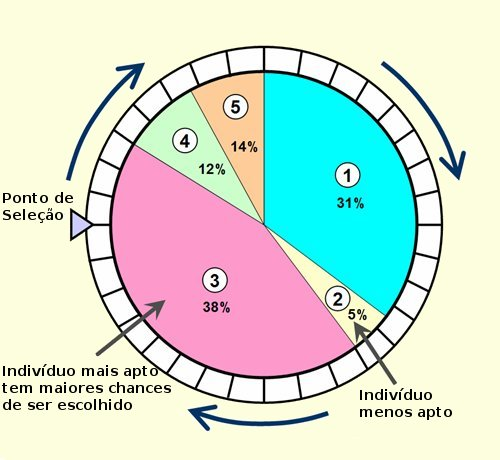
\includegraphics[scale=0.5]{images/roleta.jpg}
	\caption{Exemplo de seleção por roleta.}
	\label{fig:roleta}
\end{figure}

